% Static schematic for scan_order.pdf (make_figures.py renders it).
% Source facts: crypto 770f6a69 koblitz_orbit_dlp_fast_online.rs (mod wide):
% build_index128 order (left, right, relative); extract128_timed's wrapped scan;
% scan_state128's 166 root calls x 2 partners per state. The hit marks are
% illustrative positions, not data (data: scan_blocks.pdf).
\documentclass[tikz,border=6pt]{standalone}
\usepackage[T1]{fontenc}
\usetikzlibrary{arrows.meta,decorations.pathreplacing}
\begin{document}
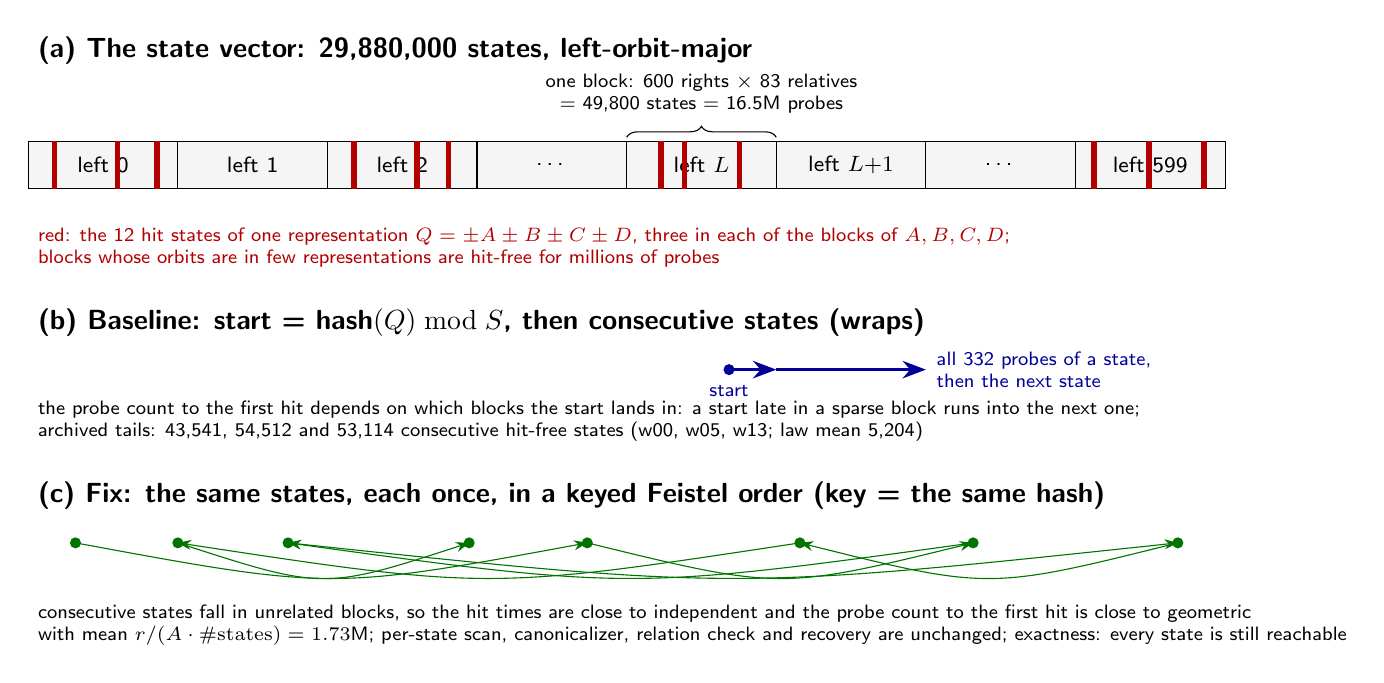
\begin{tikzpicture}[font=\sffamily\footnotesize]
  % State vector as left-orbit blocks.
  \node[anchor=west,font=\sffamily\bfseries] at (0,3.75) {(a) The state vector: 29{,}880{,}000 states, left-orbit-major};
  \foreach \b/\lab in {0/{left 0},1/{left 1},2/{left 2},3/{\ldots},4/{left $L$},5/{left $L{+}1$},6/{\ldots},7/{left 599}} {
    \draw[fill=gray!8] (\b*1.9,2) rectangle ++(1.9,0.6);
    \node at (\b*1.9+0.95,2.3) {\lab};
  }
  \draw[decorate,decoration={brace,amplitude=4pt}] (7.6,2.65) -- (9.5,2.65)
    node[midway,above=5pt,align=center,font=\sffamily\scriptsize] {one block: 600 rights $\times$ 83 relatives\\= 49{,}800 states = 16.5M probes};
  % Hits clustered by representation: 3 in each of 4 blocks.
  \foreach \x in {0.3,1.1,1.6, 4.1,4.9,5.3, 8.0,8.3,9.0, 13.5,14.2,14.9} {\fill[red!70!black] (\x,2.6) rectangle ++(0.07,-0.6);}
  \node[anchor=west,font=\sffamily\scriptsize,text=red!70!black,align=left] at (0,1.25)
    {red: the 12 hit states of one representation $Q=\pm A\pm B\pm C\pm D$, three in each of the blocks of $A,B,C,D$;\\
     blocks whose orbits are in few representations are hit-free for millions of probes};
  % Left-major scan.
  \node[anchor=west,font=\sffamily\bfseries] at (0,0.3) {(b) Baseline: start = hash$(Q) \bmod S$, then consecutive states (wraps)};
  \draw[-{Stealth},very thick,blue!60!black] (8.9,-0.3) -- (9.5,-0.3);
  \draw[-{Stealth},very thick,blue!60!black] (9.5,-0.3) -- (11.4,-0.3) node[right,font=\sffamily\scriptsize,align=left] {all 332 probes of a state,\\then the next state};
  \fill[blue!60!black] (8.9,-0.3) circle (2pt) node[below=2pt,font=\sffamily\scriptsize] {start};
  \node[anchor=west,font=\sffamily\scriptsize,align=left] at (0,-0.95)
    {the probe count to the first hit depends on which blocks the start lands in: a start late in a sparse block runs into the next one;\\
     archived tails: 43{,}541, 54{,}512 and 53{,}114 consecutive hit-free states (w00, w05, w13; law mean 5{,}204)};
  % Feistel order.
  \node[anchor=west,font=\sffamily\bfseries] at (0,-1.9) {(c) Fix: the same states, each once, in a keyed Feistel order (key = the same hash)};
  \foreach \x/\y in {0.6/0, 7.1/0, 12.0/0, 3.3/0, 14.6/0, 9.8/0, 1.9/0, 5.6/0} {\fill[green!45!black] (\x,-2.5) circle (2pt);}
  \foreach \a/\b in {0.6/7.1, 7.1/12.0, 12.0/3.3, 3.3/14.6, 14.6/9.8, 9.8/1.9, 1.9/5.6} {
    \draw[-{Stealth},green!45!black,thin] (\a,-2.5) .. controls ({(\a+\b)/2},-3.1) .. (\b,-2.5);
  }
  \node[anchor=west,font=\sffamily\scriptsize,align=left] at (0,-3.55)
    {consecutive states fall in unrelated blocks, so the hit times are close to independent and the probe count to the first hit is close to geometric\\
     with mean $r/(A\cdot\#\mathrm{states}) = 1.73$M; per-state scan, canonicalizer, relation check and recovery are unchanged; exactness: every state is still reachable};
\end{tikzpicture}
\end{document}
